\subsection{Cerebellum} \label{sub:kleinhirn} \index{Cerebellum! allgemein}
Das \textbf{Cerebellum} oder auch \textbf{Kleinhirn} gilt als wichtigstes Intergrationszentrum für die Koordination, die Feinabstimmung und auch das Erlernen von Bewegungen. Insgesamt macht es nur etwa 10~\% des Gesamtvolumens des Gehirns aus, aber es enthält mehr als 50~\% aller Neurone. Es besteht aus sich wiederholenden Teilstrukturen, die alle denselben Mikrokreislauf befolgen. Unterschiedliche Bereiche des Kleinhirns erhalten aus verschiedenen Regionen des Gehirns ihre Information und senden diese auch an andere motorische Gebiete. Daraus lässt sich schließen, dass eine ähnliche Berechnung der Informationen für unterschiedliche Bereiche des motorischens Systems im Cerebellum stattfindet \textsuperscript{\cite[Kap.~42]{kandel2013principles}}. Der genaue äußere und innere Aufbau, der Mikroverschaltung und die funktionelle Einteilung wird im Folgenden erläutert.    

\subsubsection{Lage und Morphologie}
Das Kleinhirn liegt auf der Medulla oblongata und dem Pons dorsal in der Schädelgrube. Umgeben wird es vom Tentorium cerebelli, die als eine Art Duraimitation, das Cerebellum vom Großhirn abtrennt. Die Verbindung zum Hirnstamm wird über drei symmetrische angelegte Paare an \textbf{Kleinhirnstielen} \index{Kleinhirnpedunkel} hergestellt, in denen afferente und efferente Fasern verlaufen. Sie werden als \textit{Pedunculus cerebellaris superior} (Brachium conjunctivum)\index{Pedunculus! cerebellaris superior}, \textit{Pedunculus cerebellaris medius} (Brachium medius) \index{Pedunculus! cerebellaris medius} und \textit{Pedunculus cerebellaris inferior} (Corpus restiforme) \index{Pedunculus! cerebellaris inferior} bezeichnet.  Das Dach des vierten Ventrikels wird durch die oberen und unteren Kleinhirnsegel \index{Velum} gebildet. Das Velum medullare superius zieht vom Kleinhirn zum Mesencepahlon und das Velum medullares inferius erstreckt sich ausgehend vom Cerebellum zur Medulla oblongata \textsuperscript{\cite[Kap.~7]{trepel2011neuroanatomie}}. \\
\\ \noindent Die Oberfläche weist eine extreme Faltung auf, mit vielen parallelen Furchen, genannt \textbf{Folia cerebelli}, die zur Vergrößerung der Oberfläche dienen. In die Längsrichtung lässt sich das Kleinhirn durch zwei Furchen in drei Bereiche unterteilen. Lateral liegen zwei Hemisphären, die in der Mitte über die \textbf{Vermis} (Wurm) \index{Vermis} verbunden sind. Beide cerebellaren Hemisphären setzen sich aus einer intermediären und einer lateralen Region zusammen. Zwei tiefe quer verlaufende Spalten unterteilen das Kleinhirn weiter in drei Lappen. Auf der dorsalen Oberfläche verläuft die \textit{Fissura prima}, die den \textbf{Lobus anterior} vom \textbf{Lobus posterior} abgrenzt. Diese beiden Strukturen bilden den Körper des Cerebellums. Durch die \textit{Fissura posterolateralis} auf der ventralen Oberfläche wird dieser Bereich vom \textbf{Lobus flocculonodularis} getrennt. Dieser Lappen setzt sich aus dem \textbf{Flocculus} \index{Flocculus} und dem \textbf{Nodulus} \index{Nodulus} zusammen. Der Flocculus ist eine paarige Struktur an der ventral~-~caudalen Seite, die durch den Nodulus mit dem unteren Teil des Kleinhirnwurms verbunden ist. Jeder dieser drei Lappen erstreckt sich über die gesamte Breite des Cerebellums (Abb.~\ref{fig:morph_kleinhirn}~A) \textsuperscript{\cite[Kap.~42]{kandel2013principles}}. \\
\\ \noindent Führt man einen Querschnitt durch das Kleinhirn durch, wird die grobe innere Struktur erkennbar. Außen ist ein cerebellärer Cortex, bestehend aus grauer Substanz sichtbar, der das innere Mark aus weißer Substanz umschließt. Innerhalb dieses \textbf{Kleinhirnmarklagers} befinden sich vier paarig angelegte Kleinhirnkerne, namens \textbf{Nucleus dentatus}\index{Nucleus! dentatus}, \textbf{Nucleus emboliformis}\index{Nucleus! emboliformis}, \textbf{Nucleus globosus}\index{Nucleus! globosus} und \textbf{Nucleus fastigii} \index{Nucleus! fastigii}. Der Ncl. dentatus ist der größte dieser Kerngebiete und liegt lateral in den Kleinhirnhemisphären. Medial dazu befindet sich der Ncl. emboliformis und wiederum medial dazu der Ncl. globosus. Oft werden diese beiden Bereiche auch zu einem Kern, dem \textbf{Nucleus interpositus}\index{Nucleus! interpositus} zusammengefasst. Unterhalb des Vermis in der Mitte der weißen Substanz befindet sich der Ncl. fastigii (Abb.~\ref{fig:morph_kleinhirn}~B) \textsuperscript{\cite[Kap.~7]{trepel2011neuroanatomie}}. Aus diesen Kleinhirnkernen stammt der Großteil der efferenten Fasern die aus dem Cerebellum projizieren. Eine Ausnahme bildet eine Gruppen von Purkinje-Zellen innerhalb des Lobus flocculonodularis, die direkt zu den Vestibulariskernen des Hirnstammes verlaufen \textsuperscript{\cite[Kap.~42]{kandel2013principles}}. 

\begin{figure}[H]
    \centering
    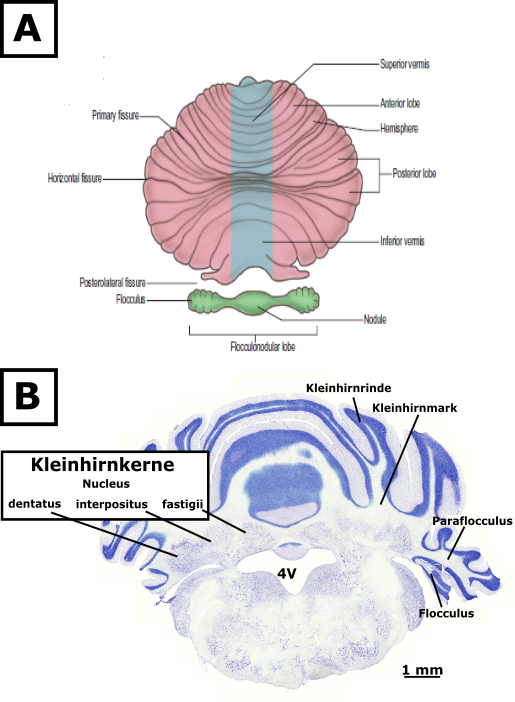
\includegraphics[width=0.7\textwidth]{pictures/Bilder_Laura/kleinhirn_ausen.png}
    \caption[Morphologie des Kleinhirns]{\textbf{Morphologie des Kleinhirns} \textbf{A:} Das Cerebellum besteht aus zwei lateralen Hemisphären, die über den Vermis in der Mitte verbunden sind. Die Fissura prima auf der dorsalen Seite des Kleinhirns grenzt den Lobus anterior von dem Lobus posterior ab. Auf der ventralen Seite verläuft die Fissura posterolateralis, die den Lobus flocculonodularis, bestehend aus Flocculus und Nodulus abtrennt. \textbf{B:} Im Querschnitt erkennt man, dass die Kleinhirnrinde das komplette Kleinhirn bedeckt. Innerhalb des Kleinhirnmarks befinden sich die Kleinhirnkerne. Von medial nach lateral sind das der Ncl. fastigii, der Ncl. interpositus und der Ncl. dentatus. Lateral am Cerebellum befindet sich der Paraflocculus und darunter der Flocculus. Nissl-Färbung (N07-1).\\ Abbildung \textbf{A} aus \textit{Neuroanatomy}, Crossman and Neary\textsuperscript{\cite[Kap.~11]{crossman2014neuroanatomy}}.}
    \label{fig:morph_kleinhirn}
\end{figure}

\subsubsection{Schichtung des cerebellären Cortex}
Der Cortex des Cerebellums lässt sich in drei Schichten unterteilen. Von innen nach außen ist das die \textbf{Körnerschicht} (\textit{Stratum granulosum}), die \textbf{Purkinje-Zellschicht} (\textit{Stratum purkinjense}) und die \textbf{Molekularschicht} (\textit{Stratum moleculare}). Innerhalb dieser Schichten liegen bestimmte Arten von Neurone, die unterschiedliche Aufgaben übernehmen \textsuperscript{\cite[Kap.~7]{trepel2011neuroanatomie}}.     

\subsubsection*{Körnerschicht} \index{Körnerschicht}
Die Körnerschicht ist die innerste Zellebene des Kleinhirncortex und gleichzeitig auch die Zellreichste. Die \textbf{Körnerzellen} bilden dabei die Mehrheit der Neurone. In histologischen Schnitten sind sie als stark gefärbte, kleine dicht gepackte Somata zu erkennen. Zusätzlich sind in dieser Schicht auch eine Vielzahl diverser Interneurone zu finden. Dazu zählen Golgi-, Lugaro-, Kandelaber- und unipolare Bürsten-Zellen. Die Körnerschicht nimmt die eingehende Informationen der unterschiedlichen motorischen Systeme in das Kleinhirn in Empfang. Dies geschieht über die \textbf{Moosfasern}, die eine der zwei Typen afferenter Kleinhirnaxone darstellen. Die Synapsen der Moosfasern bilden zusammen mit den Dendriten der Körnerzelle und den Axonen der Golgi-Zelle einen Komplex, der \textit{Glomeruli cerebellares} genannt wird. Über diesen Komplex erregen die Moosfasern diese beide Arten von Neurone (Körner-, und Golgizellen) innerhalb der Inputschicht (Abb.~\ref{fig:schichten_kleinhirn}~A,B) \textsuperscript{\cite[Kap.~42]{kandel2013principles}}.\\
Die Körnerzellen besitzen wenige kurze Dendriten. Ihre Axone sind unmyelinisiert und steigen in die äußere Molekularschicht der Kleinhirnrinde auf. Dort gabeln sie sich in sogenannte Parallelfasern, die entlang der Kleinhirnwindungen verlaufen. Sie können eine Länge von bis zu 5~mm erreichen, bevor sie dann synaptischen Kontakt mit den Dendriten der Purkinje-Zellen oder anderen Interneurone innerhalb der Molekularschicht herstellen. Der verwendete Transmitter dabei ist Glutamat. Die Golgi-Zellen auf der anderen Seite verwenden GABA und Glycin als Co-Transmitter. Damit inhibieren sie besonders die Körnerzellen als eine Art negatives Feedbacksystem \textsuperscript{\cite[Kap.~9]{paxinos2014rat}}. Der genaue Mechanismus und Schaltkreis wird in Kapitel~\ref{subsubsec:kleinhirn_schaltkreis} ausführlich erklärt. 

\subsubsection*{Purkinje-Zellschicht} \index{Purkinje-Zellschicht}
Die mittlere der drei Rindenebenen ist die Purkinje-Zellschicht. Sie besteht nur aus einer einzigen Lage an Zellkörpern der \textbf{Purkinje-Zellen} (Abb.~\ref{fig:schichten_kleinhirn}~A,B). Von dort findet auch über die Axone der Output entweder zu den Kleinhirnkernen im Marklager oder zu den Vestibulariskernen des Hirnstamms statt. An den synaptischen Endknöpfchen wird GABA als Transmitter verwendet, das eine inhibitorische Wirkung auf diese Regionen ausübt. Die Purkinje-Zellen sind mit einem Durchmesser von 50-80~$\upmu$m die größten Zellen des Cerebellums \textsuperscript{\cite[Kap.~42]{kandel2013principles}}. Nach außen hin zur Molekularschicht erstreckt sich ihr gewaltiger Dendritenbaum. Dieser erhält über mehr als 200.000 Synapsen Input, zum einen von den Parallelfasern der Körnerzellen und zum anderen auch von den \textbf{Kletterfasern}. Diese stellen die zweite Art afferenter Fasern zum Kleinhirn dar und haben ihren Ursprung ausschließlich in der unteren Olive der Medulla \textsuperscript{\cite[Kap.~7]{trepel2011neuroanatomie}}.   


\subsubsection*{Molekularschicht} \index{Molekularschicht}
Die Molekularschicht ist die äußerste Ebene des Kleinhirncortex. In ihr findet die Verarbeitung der Informationen statt. Wie oben bereits beschrieben verlaufen in ihr zum einen die Axone der Körnerzellen als \textbf{Parallelfasern} und zum anderen erstrecken sich dort die gewaltigen Dendritenbäume der Purkinje-Zellen nach außen. Die Parallelfasern sind senkrecht zu den Dentriten der Purkinje-Neurone orientiert und erstrecken sich über eine große Distanz innerhalb der Molekularschicht. Damit ist es möglich, dass eine einzelne Körnerzelle mit einer Vielzahl an Purkinje-Zellen in synaptischen Kontakt steht \textsuperscript{\cite[Kap.~42]{kandel2013principles}}. Zusätzlich befinden sich in der Molekularschicht zwei wichtige Arten GABAerger inhibitorischer Interneurone, die \textbf{Korb- und Stern-Zellen}. Die Sternzellen sind innerhalb der Molekularschicht eher nach außen hin orientiert und ihre Axone enden auf den Dendriten der Purkinje-Neurone. Die Korbzellen sind besonders innerhalb der Molekularschicht in unmittelbarer Nähe zu den Purkinje-Zellen zu finden. Ihre Axone bilden sogenannte Faserkörbe aus, die die Zellkörper der Purkinje-Zellen umschließen und synaptischen Kontakt zum Axonhügel ausbilden (Abb.~\ref{fig:schichten_kleinhirn}~A,B) \textsuperscript{\cite[Kap.~9]{paxinos2014rat}}.   


\begin{figure}[H]
    \centering
    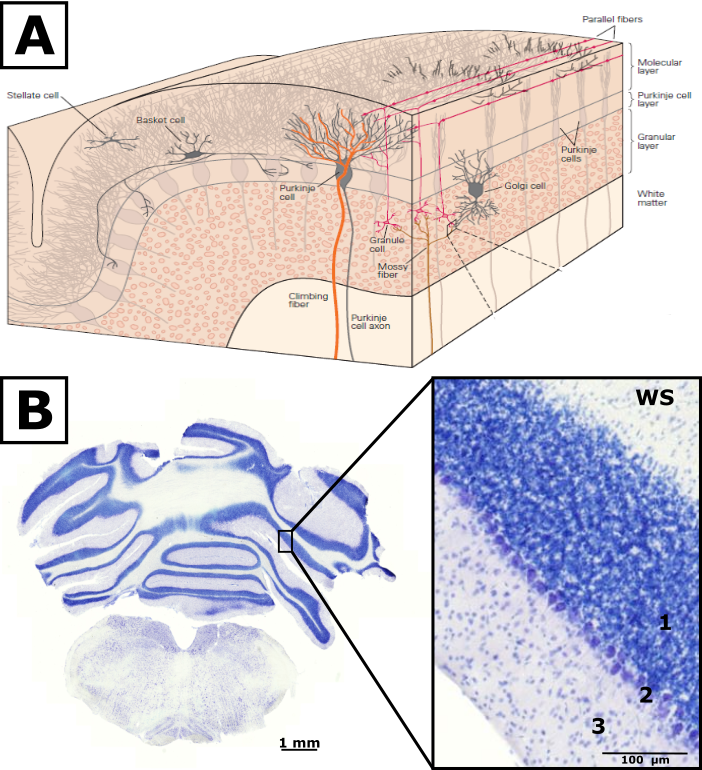
\includegraphics[width=0.9\textwidth]{pictures/Bilder_Laura/kleinhirn_schichten2.png}
    \caption[Zellschichten Kleinhirnrinde]{\textbf{Zellschichten Kleinhirnrinde.} \textbf{A:} Außen liegt die Molekularschicht mit den Parallelfasern der Körnerzellen, den Dentritenbäumen der Purkinje-Zellen, den Korbzellen und den Sternzellen. In der Mitte befindet sich die einlagige Purkinje-Zellschicht mit den Zellkörpern der Purkinje-Neurone. Die innerste Ebene ist die Körnerschicht, die Körnerzellen und Golgi-Interneuronen enthält. \textbf{B:} Querschnitt durch die Kleinhirnrinde. Von innen nach außen ist die Körnerschicht (\textbf{1}), die Purkinje-Zellschicht (\textbf{2}) und die Molekularschicht (\textbf{3}) zu erkennen. Innen ist die weiße Substanz (\textbf{WS}) des Kleinhirnmarks zu sehen. Nissl-Färbung (N04-4). \\ Abbildung \textbf{A} aus \textit{Principles of neural science}, Kandel et al. \textsuperscript{\cite[Kap.~42]{kandel2013principles}}.}
    \label{fig:schichten_kleinhirn}
\end{figure}

\subsubsection{Schaltkreis des Cerebellums} \label{subsubsec:kleinhirn_schaltkreis}
Das Kleinhirn erhält den Großteil seiner eingehenden Informationen von zwei Typen afferenter Fasern, den \textbf{Moosfasern} und den \textbf{Kletterfasern}. Es wird angenommen, dass diese beiden Systeme für eine unterschiedliche Kodierung und Verarbeitung der Informationen zuständig sind, da sie zu unterschiedlichen Cortexschichten verlaufen und auch zu einem anderem Feuerverhalten der Purkinje-Zellen führen. Über die Moosfasern wird sensorische Information aus der Peripherie und der Großhirnrinde, über Kerngebiete innerhalb der Wirbelsäule und des Hirnstamms, in das Kleinhirn geleitet. Ihre Axone enden in den Glomeruli cerebellaris der Körnerschicht. Dort erregen wenige Moosfasern eine Körnerzelle. Die weiten Ausläufer einer Zelle in Form von Parallelfasern innerhalb der Molekularschicht, erreichen daraufhin eine Vielzahl an Purkinje-Neurone. Dabei erhält ein Purkinje-Neuron nicht nur Informationen von einer Körnerzellen, sondern es wird geschätzt, dass zwischen 200.000 bis eine Millionen Körnerzellen ein Neuron kontaktieren \textsuperscript{\cite[Kap.~42]{kandel2013principles}}.\\  
Die Kletterfasern entspringen dem Ncl. olivaris inferior. Sie leiten sensorische Informationen aus der Peripherie und der Großhirnrinde weiter in das Cerebellum und projizieren dabei direkt auf die Purkinje-Neurone. Jede Zelle erhält nur von einer einzige Kletterfaser Input. Allerdings kann eine einzige Faser mit bis zu zehn Purkinje-Neuronen in Verbindung treten. Die synaptischen Endknöpfchen der Kletterfasern folgen einer topographischen Organisation. Das bedeutet, dass die Axone benachbarter Regionen der unteren Olive sagittal in Streifen der Kleinhirnrinde enden. Diese Anordnung lässt vermuten, dass die Kletterfasern die Aktivität zusammengehöriger Purkinje-Zellen präzise kontrollieren kann \textsuperscript{\cite[Kap.~42]{kandel2013principles}}.\\         
Wie bereits oben erwähnt unterscheiden sich die afferenten Fasern nicht nur in den Terminationsstellen ihrer Axone, sondern sie zeigen auch einen anderen Einfluss auf die Feuerrate der Purkinje-Zellen. Die Parallelfasern der Körnerzellen führen innerhalb der Purkinje-Zellen nur zu einer schwachen und kurzen Erregung, die als sogenannter 'simple spike' entlang das Axons hinunter wandert. Aus diesem Grund wird die erregende Aktivität vieler Parallelfasern benötigt, um die Frequenz der 'simple spikes' wesentlich zu beeinflussen. Im Ruhezustand herrscht eine spontane Aktivität von etwa 100 'simple spikes' pro Sekunde. Dies erhöht sich allerdings auf eine Feuerrate von mehreren hunderten Aktionspotentialen pro Sekunde wenn beispielsweise ein Arm oder das Gesicht willentlich bewegt wird. Indem die Feurerrate der 'simple spikes' kontrolliert wird, kodiert das System der Moosfasern die Höhe und Länge der generierten Verhaltensweisen \textsuperscript{\cite[Kap.~42]{kandel2013principles}}.\\   
Im Gegensatz dazu ist die Erregung der Purkinje-Zellen über die Kletterfasern enorm stark. Jedes Aktionspotential führt zu einer lang anhaltenden Depolarisation der Dendriten und Axone, die in einem sogenannten 'complex spike' enden. Dieser charakterisiert sich über ein anfängliches Aktionpotential mit großer Amplitude, gefolgt von einer Explosion mehrere kleinerer Aktionspotentiale. Die spontane Aktivität der Kletterfasern ist mit etwa drei 'comlex spikes' pro Sekunde im Ruhezustand sehr niedrig. Wenn die Kletterfasern jedoch aktiviert werden, stehen sie in einem zeitlichen Bezug zu bestimmten sensorischen Ereignissen. Die Feuerrate des Kletterfaser-System kodiert kaum Information. Vielmehr ist es auf das Erkennen bestimmter Ereignisse spezialisiert. Bei wichtigen Geschehnisse, synchronisieren viele Kletterfasern dennoch ihr Entladungen \textsuperscript{\cite[Kap.~42]{kandel2013principles}}.\\  
Um für eine korrekte Funktion des Schaltkreises innerhalb des Kleinhirns zu sorgen, ist der wichtigste Bestandteil, dass der inhibitorische Input mit den exzitatorischen Input innerhalb der Kleinhirnrinde und den Kleinhirnkernen verglichen wird. Das Kleinhirn kann in kleine Module eingeteilt werden. Innerhalb solch eines Moduls stehen die einzelnen Bestandteile in einer engen Beziehung. Kleinhirnkerne werden durch Purkinje-Zellen gehemmt und gleichzeitig aber durch Moos- und Kletterfasern erregt. Die Moosfasern können innerhalb eines Moduls die Kleinhirnkerne auf zwei Arten beeinflussen. Entweder direkt über einen exzitatorischen Input oder indirekt über den Cortex, indem sie die inhibitorischen Purkinje-Zellen dort aktivieren. Dieser Output moduliert damit die erregenden Signale der Moosfasern auf die Kleinhirnkerne. Gleichzeitig erhalten diese auch Input von Kollateralen der Kletterfasern. Innerhalb der Kleinhirnrinde treffen die erregenden und hemmenden Signale in den Purkinje-Zellen zusammen. Sie erhalten dabei entweder den direkten exzitatorischen Input der Parallelfasern oder diese hemmen indirekt über Verbindungen zu Interneuronen, wie den Stern-, Korb- oder Golgi-Zellen. Die Sternzellen üben dabei lokal eine inhibitorische Regulation auf die Purkinje-Zellen aus, da beide Neurone von derselben Parallelfaser erregt werden. Im Gegensatz dazu bilden die Korbzellen eine Struktur der lateralen Hemmung. Sie hemmen diejenigen Purkinje-Zellen, die benachbart zu denen liegen, die über die Parallelfaser erregt werden (Abb.~\ref{fig:schaltkreis_kleinhirn}) \textsuperscript{\cite[Kap.~42]{kandel2013principles}}.\\   
Betrachtet man das Kleinhirn im Ganzen fällt auf, dass viele Bereiche repetitive Schleifen mit dem cerebellaren Cortex bilden. Beispielsweise existieren viele reziproke Verbindungen zwischen der Kleinhirnrinde und anderen Bereichen des Cerebellums. Eine andere Schleife befindet sich innerhalb des Cortex selbst. Dort erhalten Golgi-Zellen Erregung durch die Parallelfasern. Die Axone dieser stehen über die Glomeruli cerebellaris in synaptischen Kontakt mit den Körnerzellen und Moosfasern und inhibieren darüber die Körnerzellen. Damit wird der Input der Moosfasern auf die Körnerzellen unterdrückt, was wiederum die Aktivität der Parallelfasern reguliert. Damit wird höchstwahrscheinlich eine Art Schwellenwert festgelegt, der durch den Moosfaser Input erreicht werden muss, um die Körnerzellen zu aktivieren. Eine dritte Art von Schleife beeinhaltet den Ncl. olivares inferior aus dem alle Kletterfasern hervorgehen. Aus den Kleinhirnkernen ziehen inhibitorische Fasern zu dem Komplex der unteren Olive. Wenn diese Hemmung erhöht wird, wird damit im Gegenzug der erregende Input der Kletterfasern auf die Purkinje-Zellen in der Kleinhirnrinde erniedrigt. Damit ist es dem Cerebellum möglich seinen eigenen Kletterfaser-Input zu regulieren (Abb.~\ref{fig:schaltkreis_kleinhirn}) \textsuperscript{\cite[Kap.~42]{kandel2013principles}}.\\ 
Zusätzlich wird angenommen, dass die Aktivität der Kletterfasern eine wichtige Rolle im Erlernen motorischer Fähigkeiten spielt. Sie besitzen die Fähigkeit, selektiv eine Langzeit-Depression in den Synapsen, zwischen Purkinje-Zellen und Parallelfasern, hervorzurufen, die gleichzeitig mit diesen Kletterfasern aktiviert werden. Diese Depression hält für wenige Minuten bis zu mehrere Stunden an. Eine dazu existierende Theorie besagt, dass diese Modulation der Synapsenstärke zu einer Formung bzw. Korrektur einer Augen- oder  Extremitiätenbewegung führt. Wird eine Bewegung ungenau ausgeführt, kommt es zu einem Diskrepanz Signal auf das die Kletterfasern reagieren, indem sie die Synapsenstärke der Parallelfasern unterdrücken, die damit in Verbindung stehen. Damit wird das fehlerhafte Kommando der Parallelfasern bei folgenden Bewegungen immmer stärker unterdrückt, bis ein passende Struktur an 'simple spikes' entsteht. Daraufhin verschwindet die durch die Kletterfasern ausgelöste Depression wieder \textsuperscript{\cite[Kap.~42]{kandel2013principles}}.   

\begin{figure}[H]
    \centering
    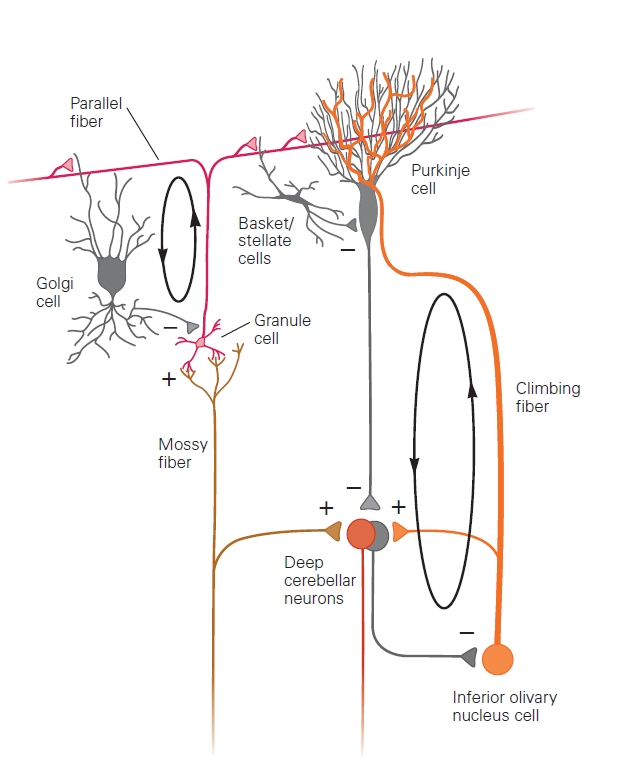
\includegraphics[width=0.6\textwidth]{pictures/Bilder_Laura/circuit-cerebellum.PNG}
    \caption[Schaltkreis der Kleinhirnrinde]{\textbf{Schaltkreis der Kleinhirnrinde.} Im Cortex des Kleinhirns und in den Kleinhirnkernen treffen die synaptische Inhibition und Erregnung der unterschiedlichen Zelltypen aufeinander. Zusammen mit den Golgi-Zellen und dem Nucleus olivaris inferior wird eine wiederkehrende Feedbackschleifen gebildet. \\ Abbildung aus \textit{Principles of neural science}, Kandel et al. \textsuperscript{\cite[Kap.~42]{kandel2013principles}}.}
    \label{fig:schaltkreis_kleinhirn}
\end{figure}

\subsubsection{Funktionelle Gliederung}
Die unterschiedlichen Bereiche des Cerebellums lassen sich auch in funktionelle Einheiten untergliedern, abhängig von ihrer Aufgabe in der Bewegungskoordination. Es wird das \textbf{Vestibulocerebellum}, das \textbf{Spinocerebellum} und das \textbf{Cerebrocerebellum} unterschieden. Zum Vestibulocerebellum zählt der Bereich des Lobus flocculonodularis. Der Vermis und die intermediären Bereiche der Hemisphären werden dem Spinocerebellum zugeordnet und das Cerebrocerebellum nimmt das Gebiet der lateralen Hemisphären in Anspruch \textsuperscript{\cite[Kap.~42]{kandel2013principles}}. Die unterschiedlichen Funktionen und Projektionen der einzelnen Bereiche werden nun detailliert besprochen. 

\subsubsection*{Vestibulocerebellum} \index{Cerebellum! Vestibulocerebellum}
Das Vestibulocerebellum erstreckt sich über den Lobus flocculonodularis, bestehend aus dem Flocculus und dem Nodulus. Es gilt als ältester und primitivster Bereich des Kleinhirns, der in Fischen das erste mal auftritt. Die eingehende Information besteht aus Parametern der Kopfbewegung und seiner relative Lage zur Schwerkraft. Dies wird in den Bogengängen und der Macula des Innenohrs gemessen. Der Großteil der afferenten Fasern des Vestibulocerebellums entstammt daher aus den Vestibulariskernen des Hirnstamms. Zusätzlich dazu erhält es auch visuellen Input. Dieser stammt entweder aus Kerngebieten des mesencephalen Prätectums unterhalb der Colliculi superiores oder aus dem primären und sekundären visuellen Cortex, die die Information über Projektionen durch die Nuclei pontis in das Kleinhirn leiten. Die Information, die über das Vestibulocerebellum verarbeitet wurde und dieses dann anschließend wieder verlässt, verläuft nicht über die Kleinhirnkerne, sondern zieht direkt zu den Nuclei vestibulares des Hirnstamms. Damit bildet es eine Ausnahme innerhalb der efferenten Projektionsbahnen des Kleinhirns, die sonst immer von den Kleinhirnkernen stammen. Der laterale Nucleus vestibularis erhält die Fasern der Purkinje-Zellen aus dem medialen Bereich des Vestibulocerebellums. Damit findet eine Modulation des lateralen und medialen Tractus vestibulospinalis statt, dessen hauptsächliche Funktion die Kontrolle der Rumpfmuskulatur und Extremitätenextensoren ist, um Gleichgewicht während Haltung und Gang zu gewährleisten.  Die Purkinje-Zellen aus den lateralen Bereichen des Vestibulocerebellums senden ihre Efferenzen zum medialen Vestibulariskern. Sie sorgen für eine Kontrolle der Augenbewegung und koordinieren die Bewegung des Kopfes zusammen mit den Augen (Abb.~\ref{fig:funktion_kleinhirn}) \textsuperscript{\cite[Kap.~42]{kandel2013principles}}.       

\subsubsection*{Spinocerebellum} \index{Cerebellum! Spinocerebellum}
Das Spinocerbellum besteht aus dem Kleinhirnwurm und den intermediären Bereichen der Hemisphären. Es erhält somatosensorische und propriozeptive Information aus der Wirbelsäule, die entweder einen direkten oder einen indirekten Verlauf zum Kleinhirn aufweisen. Wie bereits oben beschrieben (siehe Kap.~\ref{subsub:spinocerebellaris}), vermitteln  die unterschiedlichen Faserstränge des Tractus spinocerebellaris diesen Input. Wenn Interneurone aus der grauen Substanz der Wirbelsäule als Moosfasern geradewegs im Spinocerebellum enden, wird dies als direkter Weg bezeichnet. Diesen Verlauf nehmen der ventrale und dorsale spinocerebellare Trakt. Dennoch übertragen sie unterschiedliche Informationen. Über die dorsalen Fasern wird ständig Auskunft über den Status der Muskel- und Gelenkrezeptoren gegeben. Das bedeutet, die Information wird sowohl bei passiven als auch aktiven Bewegungen in das Cerebellum geleitet. Damit verschafft es sich einen Überblick über die Auswirkungen dieser. Im Gegensatz dazu überträgt der ventrale spinocerebelläre Trakt nur freiwillig ausgeführte Bewegungen. Er erhält an seinem Ausgangspunkt dieselben motorischen Anweisungen, die auch auf die Motorneurone übergehen. Damit wird dem Kleinhirn ermöglicht, die geplante Bewegung mit der tatsächlich ausgeführten Bewegung zu vergleichen und wenn nötig Korrekturen durchzuführen. Diese Bewegungsmodifikation wird nicht nur innerhalb des Spinocerebellums durchgeführt, sondern erfolgt auch bei der Koordination der Augenbewegungen durch das Vestibulocerebellum. Der indirekte Input aus der Wirbelsäule in das Kleinhirn erfolgt über verschiedene Kerngebiete innerhalb der Formatio reticularis des Hirnstamms. Dazu zählen der Nucleus reticularis lateralis medullae, Nucleus reticularis tegmenti pontis und der paramediane Nucleus reticularis \textsuperscript{\cite[Kap.~42]{kandel2013principles}}. \\ 
Die intermediären Bereiche der Hemisphären, als Bestandteil des Spinocerebellums, erhalten ihre somatosensorische Information aus den Rezeptoren der Extremitäten. Die Purkinje-Zellen, die innerhalb der intermediären Hemisphärenrinde lokalisert sind, projizieren anschließend auf den Ncl. interpositus, der sich aus dem Ncl. emboliformis und Ncl. globosus zusammensetzt. Ausgehend von diesem Kerngebiet verlässt ein Teil der efferenten Axone über den oberen Kleinhirnstiel das Cerebellum, um dann innerhalb des Nucleus ruber der contralateralen Seite zu enden. Hiervon enspringt der Tractus rubsrospinalis (siehe Kap.~\ref{subsubsec:rubrospinalis}) zur Wirbelsäule. Der andere Bestandteil efferenter Fasern aus dem Ncl. interpositus verläuft nach rostral zum Thalamus in den Nucleus ventralis lateralis (VL) (siehe Kap.~\ref{subsubsec:ncl_anterolateralis}). Aus diesem Kerngebiet verlaufen die Axone zum primären Motorcortex und nehmen darüber Einfluss auf den corticospinalen Trakt (siehe Kap.~\ref{subsubsec:corticospinalis}). Insgesamt manipuliert der intermediäre Bereich des Spinocerebellums die Muskulatur der Extremitäten und des Rumpfes \textsuperscript{\cite[Kap.~42]{kandel2013principles}}. \\   
Die eingehende Information in den Vermis ist visueller, auditorischer, vestibulärer und sensorischer Herkunft. Der somatosensorische Input stammt dabei aus dem Kopf- und Rumpfbereich des Körpers. Vom Vermis ausgehend projizieren die Neurone zum Kleinhirnkern Ncl. fastigii. Dieser wiederum sendet Axone zur Formatio reticularis und zu den lateralen Vestibulariskernen beider Seiten. Von dort verlaufen die Projektionen innerhalb des Tractus reticulospinalis und Tractus vestibulospinalis in das Rückenmark (siehe Kap.~\ref{subsubsec:reticulospinalis} und Kap.~\ref{subsubsec:vestibulospinalis}). Damit wirkt der Vermis besonders auf die Muskulatur des Rumpfes und des Kopfes während der aktiven Bewegung, um das Gleichgewicht und die Haltung zu bewahren und auch auf die Augenbewegungen. Diese Bewegung wird jedoch hauptsächlich durch das Vestibulocerebellum optimiert und nicht kontrolliert, da es eben auch viel sensorischen Input erhält (Abb.~\ref{fig:funktion_kleinhirn}) \textsuperscript{\cite[Kap.~42]{kandel2013principles}}.   

\subsubsection*{Corticocerebellum} \index{Cerebellum! Corticocerebellum}
Das Corticocerebellum erstreckt sich über den Bereich der lateralen Kleinhirnhemisphären. Die afferenten Fasern verlaufen über den mittleren Kleinhirnpedunkel und entspringen den Nuclei pontis, die wiederum ihre Informationen ausschließlich von der Großhirnrinde erhalten. Ausgehend vom Corticocerebellum projizieren die Axone der dortigen Purkinje-Zellen zum Ncl. dentatus. Die Fasern dieses Kerngebiets verlassen das Kleinhirn über den Pedunculus cerebellaris superior und enden entweder im ventrolateralen Thalamus oder im Ncl. ruber. Beide Fasertrakte kreuzen dabei auf die contralaterale Seite. Vom Ncl. ventralis lateralis entspringen Fasern, die zu motorischen Arealen des Großhirns ziehen (Kap.~\ref{subsubsec:ncl_anterolateralis}). Innerhalb des Ncl. ruber enden die efferenten Fasern des Ncl. dentatus in einem bestimmten parvozellulären Bereich. Diese Region entsendet Axone zum Nucleus olivaris inferior, der dann wiederum zum Kleinhirn in Form von Kletterfasern projiziert (Kap.~\ref{subsubsec:untere_olive}). Damit entsteht eine wiederkehrende Schleife an Informationen. Da die parvozelluläre Zone innerhalb des Ncl. ruber auch Input aus dem prämotorischen Cortex erhält, liegt die Vermutung nahe, dass diese Rückkopplungsschleife zur mentalen Wiederholung von Bewegungen und auch zum motorischen Lernen fungiert. Im Großen und Ganzen besteht die Hauptfunktion der lateralen Hemisphären, aufgrund ihrer reziproken Verbindung zum Motorcortex, in der Planung und Ausführung von Bewegungen \textsuperscript{\cite[Kap.~42]{kandel2013principles}}.\\
Das Corticocerebellum ist evolutionär gesehen am jüngsten. Im Vergleich zu Katzen und Affen ist es in Menschen und Menschenaffen sogar deutlich vergrößert. Im Bezug auf das vergrößerte Großhirn in Menschen und basierend auf neuen Studien wird vermutet, dass es sogar eine Rolle in Wahrnehmungsprozessen und kognitiven Funktionen spielt (Abb.~\ref{fig:funktion_kleinhirn}) \textsuperscript{\cite[Kap.~42]{kandel2013principles}}. 

\begin{figure}[H]
    \centering
    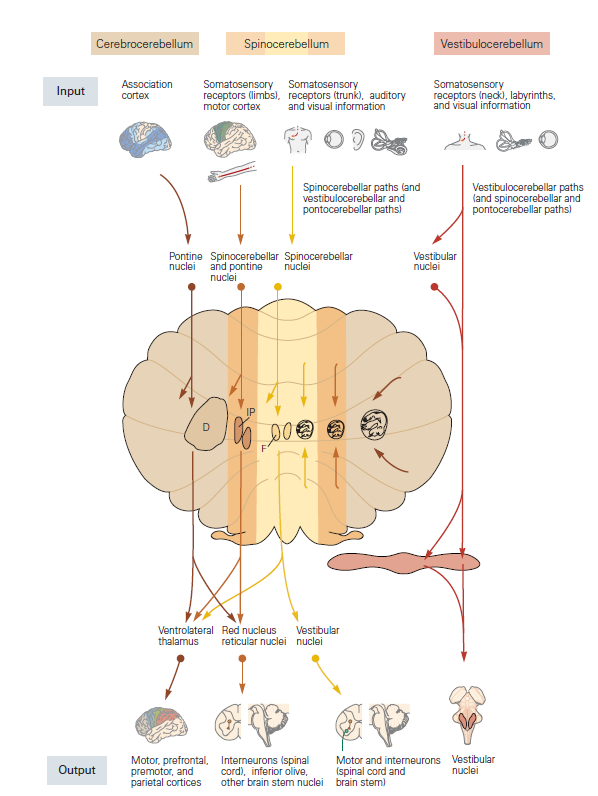
\includegraphics[width=\textwidth]{pictures/Bilder_Laura/funktionelle_einteilung_kleinhirn.PNG}
    \caption[Funktionelle Einteilung des Kleinhirns]{\textbf{Funktionelle Einteilung des Kleinhirns.} Das Kleinhirn lässt sich funktionell in das Vestibulocerebellum, das Spinocerebellum und das Corticocerebellum unterteilen. Diese Regionen erhalten aus unterschiedlichen motorischen Gebieten ihren Input und projizieren zu verschiedenen Zielgebieten. Somit unterscheiden sie sich in ihrer Funktion. D: Ncl. dentatus; IP: Ncl. interpositus; F: Ncl. fastigii. \\ Abbildung aus \textit{Principles of neural science}, Kandel et al. \textsuperscript{\cite[Kap.~42]{kandel2013principles}}.}
    \label{fig:funktion_kleinhirn}
\end{figure}

